\documentclass[compress]{beamer}

\usetheme{Szeged}
\RequirePackage[T1]{fontenc}
\RequirePackage[utf8]{inputenc}
\RequirePackage[frenchb]{babel}
\usepackage[babel=true,kerning=true]{microtype}
\usepackage{tikz,listings,algorithm,algorithmic,booktabs}
\usetikzlibrary{automata,shapes,snakes,arrows}

\tikzstyle{every picture}=[sibling distance=3cm, shorten >=1pt, node distance=2cm,%
	>=stealth', bend angle=10, auto, initial text=]

\title[SEM IN310 - SH]{Systèmes Hybrides\\
	IN310 - Modèles de systèmes embarqués}
\author[Charles Lesire]{Charles Lesire-Cabaniols (ONERA / DCSD)\\{\tt charles.lesire@onera.fr}}
\date[2010-2011]{3A-SEM - 2010-2011}

\graphicspath{{../figures/}}
\lstset{basicstyle=\tiny,tabsize=2,%frame=single,%
	emph={define,domain,requirements,strips,typing,types,predicates,
		action,parameters,precondition,vars,effect,objects,init,goal},%
	emphstyle=\bf}

\begin{document}

\begin{frame}
\titlepage
\end{frame}

\begin{frame}
\tableofcontents[hidesubsections]
\end{frame}

%%%%% INTRODUCTION %%%%%
\section{Systèmes Hybrides}
\subsection{Rappel}
\begin{frame}
\tableofcontents[currentsection]
\end{frame}

\begin{frame}{Types de variables}
Le modèle mathématique d'un système est caractérisé par :
\begin{itemize}
\item la nature de ses \structure{variables d'état}  :
	\begin{itemize}
	\item variables \structure{continues} :  prennent leurs valeurs sur le domaine des réels ${\cal R}$.
	\item variables \structure{discrètes} :  prennent leurs valeurs sur un domaine représenté par un ensemble  dont le nombre d'éléments est fini (ex: les  entiers naturels ${\cal N}$, variables booléennes)/
	\end{itemize} 
\item la nature de la variable indépendante qui représente le \structure{temps}
\end{itemize}
\end{frame}

\begin{frame}{Types de systèmes}
\begin{columns}
\column{.5\textwidth}
	\begin{block}{Systèmes continus}
	\begin{itemize}
	\item temps : variable continue (temps dense)
	\item variables d'état continues, évolution dictée par le temps
	\item équations algébro-différentielles $\overset{.}{x}(t)=Ax(t)+Bu(t)$, transformée de Laplace
	\item Ex : température d'une pièce
	\end{itemize}
	\end{block}
\column{.5\textwidth}
	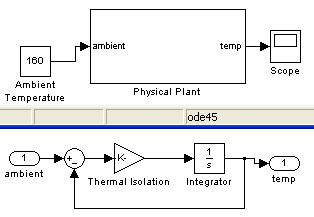
\includegraphics[width=.9\linewidth]{plant_sans}
\end{columns}
\end{frame}

\begin{frame}{Types de systèmes}
\begin{columns}
\column{.5\textwidth}
	\begin{block}{Systèmes échantillonnés}
	\begin{itemize}
	\item temps : variable discrète\\
		{\scriptsize $\theta_0$, $\theta_1$ \ldots $\theta_{n-1}$ $\theta_n$, $\theta_{n+1}$ \ldots}
	\item variables d'état continues ({\it observées} à $\theta_i$)%\\
	\item équations aux différences $X_{k+1}=A_k.X_k+B_kU_k$, transformée en Z
	\end{itemize}
	\end{block}
\column{.5\textwidth}
	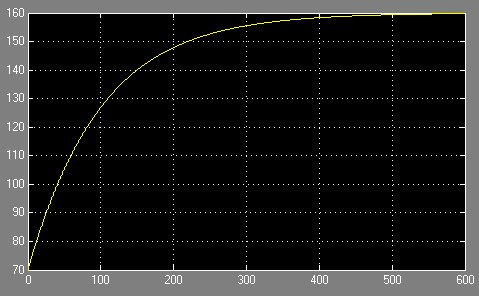
\includegraphics[width=.9\linewidth]{xy_temp_s}
\end{columns}
\end{frame}

\begin{frame}{Types de systèmes}
\begin{block}{Systèmes à événements discrets}
	\begin{itemize}
	\item représentés par une suite d'{\it événements discrets} (ex: un plan)
	\item temps : relation de précédence
	\item variables d'état discrètes : valeur x(k+1) calculé directement à partir de x(k), sans 		considérer le temps (fonction des événements)
	\item automates, réseaux de Petri
	\item ex : nombre de pièces dans un système de manufacture
	\end{itemize}
\end{block}
\end{frame}

\begin{frame}{Types de systèmes}
\begin{columns}
\column{.6\textwidth}
	\begin{block}{Systèmes discrets}
	\begin{itemize}
	\item temps : variable continue (temps dense)
	\item variables d'état discrètes (ex: machine libre ou occupée, ventilateur ON/OFF)
	\item automates (temporisés), réseaux de Petri (temporels)
	\end{itemize}
	\end{block}
\column{.4\textwidth}
	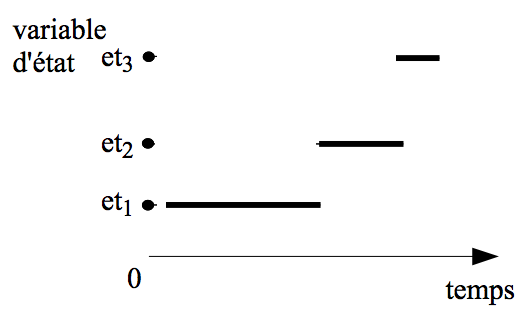
\includegraphics[width=.9\linewidth]{discret1}
\end{columns}
\end{frame}

\begin{frame}{Types de systèmes}
\begin{block}{Systèmes hybrides}
	\begin{itemize}
	\item évolution à la fois en fonction 
		\begin{itemize}
		\item du temps continu  et
		\item des événements discrets
		\end{itemize}
	\item  variables d'état continues et  variables d'état discrètes
	\item automates hybrides, réseaux de Petri hybrides ; Simulink et  StateFlow
	\end{itemize}
\end{block}
\end{frame}

%%%%% SH %%%%%
\subsection{Historique}
\begin{frame}{Systèmes Hybrides}
\begin{itemize}
\item Evolution technologique :
	\begin{itemize}
	\item systèmes distribués, réseaux : sous-systèmes interconnectés ;
	\item 98\% des microprocesseurs sont intégrés sur des systèmes physiques : BMW (72 $\mu$P en réseau), Boeing 777 (1280 $\mu$P en réseau) ;
	\item avancées sur les technologies de capteurs et d'actionneurs
	 \end{itemize}
\item 2 visions:
	\begin{itemize}
	\item \structure{Théorie du Contrôle}: systèmes continus, controllabilité, stabilité, atteignabilité, robustesse, \dots Résultats en modélisation : switched control system, supervisory control system, piecewise affine systems (PWA)
	\item \structure{Informatique} : systèmes de état-transition, composition et abstraction, concurrence, \dots Résultats en modélisation : automates hybrides, réseaux de Petri hybrides
	\end{itemize}
\end{itemize}
\end{frame}

\begin{frame}{Systèmes Hybrides}
\begin{itemize}
\item juin 1991 : First workshop on Hybrid Systems, R.L. Grossman and A. Nerode, Cornell University, USA
\item oct. 1992: 2nd workshop, Technical University of Lyngby, Danemark
\item 1993 : Hybrid Systems (Grossman et al.), Lecture Notes in Computer Science
\item avril 1998 : First Hybrid Systems: Computationand Control (HSCC) (Henzinger and Sastry), Berkeley
\item 2003 : IFAC conference on Analysis and Design of Hybrid Systems (ADHS), France
\item de nombreux problèmes ouverts : modélisation, analysé, vérification, synthèse de controleur, simulation, génération de code, complexité, \dots
\end{itemize}
\end{frame}

%%%%% AUTOMATES HYBRIDES %%%
\section{Automates Hybrides}
\begin{frame}
\tableofcontents[currentsection]
\end{frame}

\subsection{Introduction}
\begin{frame}{Automates hybrides}
\begin{itemize}
\item Les \structure{automates temporisés} décrivent un type de systèmes hybrides
\item Automates hybrides pour représenter des horloges \structure{asynchrones} !
\item \`A l'origine : Alur, Henzinger, Sifakis, Yovine, \dots
\item \'Ecole française performante : Sifakis, Yovine, Maler (VeriMAG), Asarin (LIAFA / Paris 7)
\item Inspiration d'un cours de Claire Tomlin (\url{http://www.stanford.edu/class/aa278a/})
\item Références, approfondissemnets $\rightarrow$ "Google is your friend!"
\end{itemize}
\end{frame}

\begin{frame}{Exemples}{Bouncing ball}
\begin{columns}
\begin{column}{0.35\linewidth}
	\begin{tikzpicture}
	\setlength{\arrayrulewidth}{1pt}
	\node[state] (q) {$\begin{array}{c}q_0\\%
		\addlinespace \toprule
		\dot{x}_1 = x_2\\%
		\dot{x}_2 = -g\\%
		x_1 \geq 0%
		\end{array}$};
	\path (q) edge [loop above] node {$\begin{array}{c}%
		x_1 = 0 \wedge x_2 \leq 0\\%
		x_2 := -c \, x_2%
		\end{array}$} (q);
	\end{tikzpicture}
\end{column}
\begin{column}{0.65\linewidth}
	\begin{itemize}
	\item $x_1$ : position verticale de la balle ;
	\item $x_2$ : vitesse vertical de la balle ;
	\item $g$ : accélération ;
	\item $c \in [0, 1]$ : coefficient de restitution ;
	\item transitions discrètes lors des rebonds ;
	\item Propriétés :
		\begin{itemize}
		\item non-bloquant ;
		\item si $c < 1$, l'automate est \structure{Zénon}.
		\end{itemize}
	\end{itemize}
\end{column}
\end{columns}
\end{frame}

\begin{frame}{Exemples}{Pilote automatique}
\begin{center}
	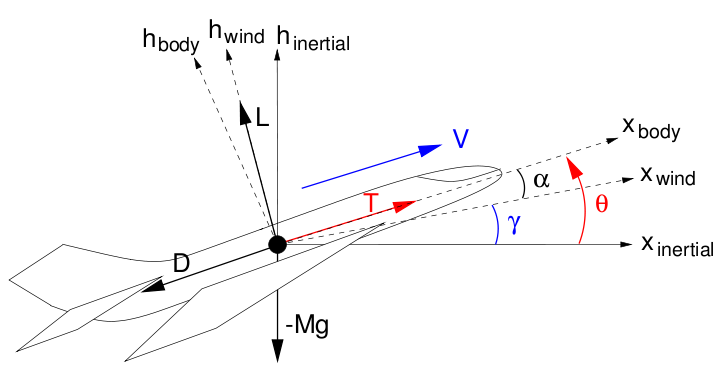
\includegraphics[width=.4\linewidth]{aircraft}
\end{center}
\begin{columns}
	\begin{column}{0.4\linewidth}
	\begin{tikzpicture}[scale=.8,transform shape]
	\node[state] (q1) at (0,0) {$q_1$};
	\node[state] (q2) at (1.5,-1) {$q_2$};
	\node[state] (q3) at (1,-2.5) {$q_3$};
	\node[state] (q4) at (-1,-2.5) {$q_4$};
	\node[state] (q5) at (-1.5,-1) {$q_5$};
	\foreach \x in {q1,q2,q3,q4,q5} {
		\foreach \y in {q1,q2,q3,q4,q5} {
			\ifthenelse{\equal{\x}{\y}}{}{%
				\path (\x) edge[->, bend right] (\y);
			}
		}
	}
	\end{tikzpicture}
\end{column}
\begin{column}{0.6\linewidth}
	\begin{itemize}
	\item Équations de la dynamique du vol,
	\item \structure{Modes} de vol, i.e. \structure{stratégies} de contrôle.
	\end{itemize}
\end{column}
\end{columns}
\end{frame}

\subsection{Définitions}
\begin{frame}{Automates Hybrides}
Un \structure{Automate hybride} (autonome) est défini par :
\begin{itemize}
\item un ensemble d'états discrets $Q$,
\item un espace d'état continu $X \subset \mathbb{R}^n$,
\item un ensemble d'état initiaux $Init \subset Q \times X$,
\item des invariants $Inv \subset Q \times X$,
\item une dynamique continue $f: Q \times X \rightarrow X$,
\item une dynamique discrète $R: Q \times X \rightarrow 2^{Q \times X}$.
\end{itemize}
\end{frame}

\begin{frame}{Comportement dynamique d'un AH}
Une succession de \structure{phases} séparées par des \structure{événements}
\begin{itemize}
\item au cours d'une phase : les variables discrètes n'évoluent pas ; les variables continues
	évoluent continûment dans le temps
\item lors d'un événement :  les variables discrètes évoluent ; les variables continues peuvent
	changer de valeur ($\leadsto$ discontinuité, variable non dérivable en ce point)~; la
	structure du modèle continu peut être modifiée!!
\end{itemize}
\end{frame}

\begin{frame}{Ensemble temporel hybride}
Un \structure{ensemble temporel hybride} (Hybrid Time Set) est une séquence d'intervalles $\tau = \{I_i\}_{i \geq 0}$ telle que $\forall \, i$ :
\begin{itemize}
\item $I_i = [\tau_i, \tau_i']$
\item $\tau_i \leq \tau_i' = \tau_{i+1}$
\end{itemize}
\vspace{1cm}
\begin{itemize}
\item $<\tau> = \sup i$ ($N$ ou $+\infty$) ; 
	$\displaystyle ||\tau|| = \sum_{i=0}^{<\tau>} (\tau_i' - \tau_i)$
\item si $<\tau> = \infty$ et $||\tau|| < \infty$, $\tau$ est Zénon.
\end{itemize}
\end{frame}

\subsection{Trajectoire}

\begin{frame}{Trajectoire hybride}
L'exécution d'un automate hybride est une \structure{trajectoire hybride} $(\tau, q, x)$ telle que :
\begin{itemize}
\item $(q_0, x_0) \in Init$,
\item $(q_{i+1}(\tau_{i+1}), x_{i+1}(\tau_{i+1})) \in R((q_i(\tau_i'), x_i(\tau_i')))$,
\item $\forall \, i$ :
	\begin{itemize}
	\item $q_i : I_i \rightarrow Q$ est constante (i.e., $q_i(t) = q_i(\tau_i) \forall t \in I_i$),
	\item $x_i : I_i \rightarrow X$ est une solution de l'équation différentielle 
		$$\dot{x}_i = f(q_i(t), x_i(t))$$
	\item $\forall \, t \in [\tau_i, \tau_i'[, \, x_i(t) \in Inv(q_i(t))$.
	\end{itemize}
\end{itemize}
\end{frame}

%%%%% PROPS %%%%
\section{Propriétés}
\begin{frame}
\tableofcontents[currentsection]
\end{frame}

\subsection{Trajectoires}
\begin{frame}{Propriétés}{Trajectoires}
\begin{block}{Non-bloquant}
Un automate hybride est \structure{non-bloquant} si $\forall \, (q_0, x_0) \in Init$, il existe une trajectoire infinie partant de $(q_0, x_0)$.
\end{block}
\begin{block}{Déterminisme}
Un automate hybride est \structure{déterministe} si $\forall \, (q_0, x_0) \in Init$, il existe au plus une trajectoire \structure{maximale} partant de $(q_0, x_0)$.
\end{block}
\end{frame}

\begin{frame}{Propriétés}{Trajectoires}
Dans le cas continu :
\begin{itemize}
\item non-bloquant $\Leftarrow$ $f$ continue
\item déterministe $\Leftarrow$ $f$ lipschitzienne
\end{itemize}
Dans le cas hybride :
\begin{itemize}
\item Plus de "souplesse" : une transition discrète peut débloquer l'automate !
\item non-bloquant 
	$\Leftarrow \forall (q, x) \in Trans \cap Reach, \exists \, q' \in Q \, / \, R(q, x) = (q', x')$
	\begin{itemize}
	\item $Trans$ ensemble des \structure{états de transition} : l'équation différentielle n'admet pas de solution dans l'invariant ;
	$$Q \times Inv \mbox{ ouvert et } f \mbox{ localement lipshitzienne } \Rightarrow Trans = (Q \times Inv)^c$$
	\end{itemize}
\end{itemize} 
\end{frame}

\subsection{Zénon}
\begin{frame}{Propriétés}{Zénon}
Un automate est \structure{Zénon} si pour $(q_0, x_0) \in Init$, toutes les trajectoires infinies $\tau$ depuis $(q_0, x_0)$ sont Zénon :
\begin{itemize}
\item $<\tau> = \infty$
\item $||\tau|| < \infty$
\end{itemize}
\vspace{1cm}
Du à la modélisation du système, qui est une abstraction du système réel.\\
Pose des problèmes pour la simulation (et donc pour la vérification).
\end{frame}

\begin{frame}{Propriétés}{Zénon}
\begin{block}{Régularisation}
On peut \structure{régulariser} un automate hybride Zénon $H$ en construisant une famille d'automates $H_{\epsilon}$.
\begin{itemize}
\item $\phi : Q_{\epsilon} \times X_{\epsilon} \rightarrow Q \times X$ fait correspondre un état de $H_{\epsilon}$ à un état de $H$ ;
\item $H_{\epsilon}$ "tend vers $H$" quand $\epsilon \rightarrow 0$.
\end{itemize}
\end{block}
\end{frame}

\begin{frame}{Propriétés}{Zénon}
\begin{tikzpicture}
\setlength{\arrayrulewidth}{1pt}
\node[state] (q1) {$\begin{array}{c}q_1\\%
	\addlinespace \toprule
	\dot{x}_1 = 0\\ \dot{x}_2 = 0\\ \dot{x}_3 = 1\\ x_3 \leq \epsilon%
	\end{array}$};
\node[state] (q0) [left of=q1, node distance=7cm] {$\begin{array}{c}q_0\\%
	\addlinespace \toprule
	\dot{x}_1 = x_2\\ \dot{x}_2 = -g\\ \dot{x}_3 = 0\\ x_1 \geq 0%
	\end{array}$};
\path (q0) edge [->,bend right] node[below=1.2cm] {\small $\begin{array}{c}%
	x_1 < 0 \vee (x_1 = 0 \wedge x_2 \leq 0)\\ x_3 := 0%
	\end{array}$} (q1);
\path (q1) edge [->,bend right] node[above=1.2cm] {\small $\begin{array}{c}%
	x_3 \geq \epsilon\\ x_2 := -c \, x_2%
	\end{array}$} (q0);
\end{tikzpicture}
$$\phi(q_0, (x_1, x_2, x_3)) = \phi(q_1, (x_1, x_2, x_3)) = (q, (x_1, x_2))$$
\end{frame}

\subsection{Accessibilité}
\begin{frame}{Propriétés}{États}
\begin{block}{Accessibilité}
Un état $(q, x) \in Q \times X$ est \structure{accessible} s'il existe une trajectoire \structure{finie} $\sigma$ qui finie en $(q, x)$ (i.e. $<\tau> = N < \infty$ et $(q_N(\tau_N'), x_N(\tau_N')) = (q, x)$).
\end{block}
\begin{block}{Invariants}
L'ensemble $M \subset Q \times X$ est appelé \structure{invariant} si $\forall \, (q_0, x_0) \in M$ et pour toute trajectoire $\sigma$ partant de $(q_0, x_0)$ :
$$ \forall \, i, \; \forall \, t \in I_i, \; (q_i(t), x_i(t)) \in M$$
\end{block}
\end{frame}

\begin{frame}{Automates hybrides rectangulaires}
\begin{block}{Rectangle}
Un ensemble $R \subset \mathbb{R}^n$ est un \structure{rectangle} si $R = \Pi_{i=1}^n R_i$ où $R_i$ est un intervalle dont les bornes sont rationnelles.
\end{block}
\begin{block}{Automate rectangulaire}
Un \structure{automate rectangulaire} est un automate hybride tel que :
\begin{itemize}
\item $Q = \{q_1, \dots, q_m\}$ ;
\item $Init = \bigcup_{i=1}^m \{q_i\} \times Init(q_i)$ où $Init(q_i)$ est un rectangle ;
\item $f(q,x) = F(q)$ où $F(q)$ est un rectangle ;
\item $Inv(q)$ est un rectangle.
\end{itemize}
\end{block}

$\longrightarrow$ Automates rectangulaires initialisés : plus grande classe d'AH pour laquelle l'accessibilité est \structure{décidable} (mais PSPACE) !
\end{frame}

\subsection{Stabilité}
\begin{frame}{Stabilité}
\begin{block}{Equilibre}
L'état continu $x_e$ est un \structure{point d'équilibre} de $H$ si :
\begin{itemize}
\item $f(q, x_e) = 0$ pour tout $q \in Q$ ;
\item $R(q, x_e) \subset Q \times \{x_e\}$.
\end{itemize}
\end{block}
\begin{block}{Equilibre stable}
L'état continu $x_e$ est un point d'équilibre \structure{stable} si $\forall \epsilon > 0, \, \exists \delta > 0$ tel que pour toute trajectoire $(\tau, (q, x))$ partant de $(q_0, x_0)$,
$$ ||x_0 - x_e|| < \delta \Rightarrow \forall t \in \tau, \, || x(t) - x_e || < \epsilon $$
\end{block}
$x_e$ stable pour $f(q)$, pour tout $q$ $\not\Rightarrow$ $x_e$ stable pour $H$ !!\\
\small même si les variables ne sont pas réinitialisés ($R(q,x) \subset Q \times \{x\}$)
\end{frame}

\begin{frame}{Stabilité}
\begin{block}{Théorème de Lyapunov pour les SH}
Soit $H$ un automate tel que $x_e$ est un point d'équilibre et $R(q,x) \in Q \times \{x\}, \forall q$.
Soit $D$ un ouvert de $\mathbb{R}^n$ tel que $x_e \in D$. $x_e$ est stable s'il existe $V : D \rightarrow \mathbb{R}$ une fonction $C^1$ telle que :
\begin{itemize}
\item $V(x_e) = 0$
\item $V(x) > 0 \forall x \in D \backslash \{(x_e)\}$
\item $\frac{\partial V(x)}{\partial x} f(q,x) \leq 0, \forall x \in D, \forall q \in Q$
\end{itemize}
\end{block}
\begin{block}{Système linéaire par morceaux}
Pour un système linéaire par morceaux, i.e. $f(q_i, x) = A_i x$. $x_e$ est stable s'il existe une solution $P$ symétrique définie positive au système de LMI
	$$\forall i, \; A_i^T P + P A_i < 0$$
\end{block}
\end{frame}

%%%%% USAGE %%%%%
\section{Utilisations}
\begin{frame}
\tableofcontents[currentsection]
\end{frame}

\subsection{Contrôle}
\begin{frame}{Contrôle}{Automate hybride}
Un \structure{automate hybride} $H$ est défini par :
\begin{itemize}
\item $Q$, $X$,
\item $Init \subset Q \times X$ un ensemble d'états initiaux,
\item $In$ un ensemble fini de variables d'entrées, $In = \Sigma \cup W$,
	\begin{itemize}
	\item $\Sigma = \Sigma_U \times \Sigma_D$, avec $\Sigma_U$ les entrées discrètes et $\Sigma_D$ les perturbations discrètes,
	\item $W = U \times D$, avec $U$ les entrées continues (contrôlables) et $D$ les perturbations continues (bruits),
	\end{itemize}
\item $f : Q \times X \times W \rightarrow \mathbb{R}^n$ un champ vectoriel,
\item $Inv : Q \rightarrow 2^{X \times W}$ les invariants de $H$,
\item $R : Q \times X \times In \rightarrow 2^{Q \times X}$ la fonction de transition,
\item $Out = P \cup Y$ l'ensemble des variables de sortie, discrètes ($P$) et continues ($Y$).
\end{itemize}
\end{frame}

\begin{frame}{Contrôle}{Hypothèses}
On fait les hypothèses suivantes :
\begin{itemize}
\item $f$ est \structure{lipshitzienne} sur $X$ et continue sur $W$ ;
\item $\forall q, \; Inv(q)$ est un ouvert ;
\item $\forall (q, x), \forall (\sigma_u, u) \in \Sigma_U \times U, \; 
	\exists (\sigma_d, d) \in \Sigma_D \times D$ tel que
	$$(x, (\sigma_u, \sigma_d), (u, d)) \in Inv(q) \; \vee \; R(q, x, (\sigma_u, \sigma_d), (u, d)) \neq \emptyset$$
\end{itemize}
\end{frame}

\subsection{Algorithme}
\begin{frame}{Contrôle}{Principe}
On veut satisfaire une propriété de sûreté, i.e. calculer l'invariant contrôlé maximal $F_C \subset F \subset Q \times X$.\\
On appréhende le problème comme un \structure{jeu}, dans lequel :
\begin{itemize}
\item les perturbations essaient de fuir $F$ en
	\begin{enumerate}
	\item faisant des \structure{sauts} (discrets) hors de $F$,
	\item \structure{tirant} (continument) le système hors de $F$ ;
	\end{enumerate}
\item le contrôleur essaie de rester dans $F$ en
	\begin{enumerate}
	\item \structure{tirant} le système dans $F$ (en évitant les sauts),
	\item faisant des \structure{sauts} dans $F$ (évitant les sorties continues).
	\end{enumerate}
\end{itemize}
\end{frame}

\begin{frame}{Contrôle}{Principe}
\begin{itemize}
\item $Pre_u : 2^{Q\times X} \rightarrow 2^{Q\times X}$ prédécesseurs contrôlables : une action contrôlable peut forcer à rester dans $K$
$$\scriptstyle Pre_u(K) = \{(q,x)\in K / \exists u \in In_U, \forall d \in In_D, \; (x, u, d) \not\in Inv(q) \wedge R(q, x, u, d) \subset K \}$$
\item $Pre_d : 2^{Q\times X} \rightarrow 2^{Q\times X}$ prédécesseurs incontrôlables : des actions incontrôlables peuvent forcer à sortir de $K$
$$\scriptstyle Pre_d(K) = \{(q,x)\in K / \forall u \in In_U, \exists d \in In_D, \; R(q, x, u, d) \cap K^c \neq \emptyset \} \cup K^c$$
\item $Reach : 2^{Q\times X} \times 2^{Q\times X} \rightarrow 2^{Q\times X}$ : états depuis lesquels $G$ est accessible sans atteindre $E$
\end{itemize}
$$\scriptstyle \!\!\!\!\!\!
Reach(G, E) = \{(q(0),x(0)) / \forall u \in \mathcal{U}, \exists d \in \mathcal{D}, \; (q(t),x(t)) \in G \mbox{ and } (q(s),x(s)) \in Inv \backslash E \, \forall s \in [0, t]\}$$
\small où $(q(s),x(s))$ est la trajectoire d'équation $\dot{x} = f(q(s), x(s), u(s), d(s))$.
\end{frame}

\begin{frame}{Contrôle}{Principe}
\begin{block}{Algorithme}
Point fixe de l'équation :
\begin{eqnarray*}
W^0 &=& F\\
W^{i-1} &=& W^i \backslash Reach(Pre_d(W^i), Pre_u(W^i))
\end{eqnarray*}
\end{block}
Calcul de $Pre$ : inversion de la fonction $R$.\\
Calcul de $Reach$ : résolution d'un équation d'\structure{Hamilton-Jacobi} sous contrainte.\\
$\rightarrow$ algorithme semi-décidable pour des \structure{automates hybrides linéaires}\\
\small $\qquad f$ linéaire en $x$, gardes et resets ($R$) polyédriques
\end{frame}

\subsection{Filtrage}
\begin{frame}{Filtrage}
\`A partir des observations $y$ de l'état \structure{continu}, estimer l'état \structure{hybride} $(\hat{q}, \hat{x})$.\\
Approches :
\begin{itemize}
\item Filtres de Kalman étendus sur des automates hybrides probabilistes concurrents (Hofbaur \& Williams, 2004)\\
\item \structure{Filtrage particulaire} sur automates hybrides (Koutsoukos {\it et al.}, 2006; Funiak \& Williams, 2003; Pfeffer \& Dearden, 2007; \dots)
\item Filtre ensembliste sur automates hybrides (Benazera, 2004).
\end{itemize}
\end{frame}

\subsection{Outils}
\begin{frame}{Outils}
\begin{itemize}
\item HyTech (U. Berkeley) : vérification de propriété temporelle (LTL) sur des automates hybrides linéaires (composés) ;
\item $d/dt$ (VeriMAG) : accessibilité dans les AH linéaires ; synthèse de contrôleur discret ;
\item CHARON (U. Pennsylvanie) : hiérarchisation, simulation.
\end{itemize}
\end{frame}

\end{document}
